\hypertarget{einleitung-motivation}{%
\section{Einleitung \& Motivation}\label{einleitung-motivation}}

Die Clusteranalyse ist ein Verfahren des maschinellen Lernens, bei dem
in einem Datenset nach ``Ähnlichkeitsgruppierungen'' gesucht wird
\autocite[Kap. 5.2.3 Unüberwachtes Lernen]{papp2019}. Die einzelnen
Objekte eines Datensets werden dabei von einem Clustering-Algorithmus in
Gruppen sortiert, ``{[}\ldots{]} sodass sich die Individuen innerhalb
einer Gruppe auf eine Art und Weise ähnlich sind und unähnlich denen in
anderen Gruppen'' \autocite[Kap. 1.1 What Is a Cluster?]{king2015}. Mit
Hilfe dieser gefundenen Gruppen oder Cluster können im Anschluss neue
Erkenntnisse und Anwendungen abgeleitet werden. \autocite[Kap. 5.2.3
Unüberwachtes Lernen]{papp2019}

Speziell im Bereich E-Commerce wurde die Clusteranalyse z.B. für die
Entwicklung von Empfehlungsalgorithmen verwendet (\autocite{oh2019},
\autocite{cui2021} und \autocite{kumar2001}). Ebenso gibt es eine
interessante Arbeit von Kou und Lou \autocite{kou2012}, welche mithilfe
von Clusteranalyse die Suchergebnisse einer Web-Suchmaschine
verbesserten.

Inspiriert durch diese Ansätze beschäftigte sich der Autor nun mit der
Frage, ob es sinnvolle Anwendungen für die Clusteranalyse im
Zusammenhang mit Product-Information-Management-Systemen (PIM-Systemen)
gibt. Dabei handelt es sich um spezielle IT-Systeme, welche i.d.R. im
Zentrum der Architektur von E-Commerce-Unternehmen zu finden sind. Sie
fungieren als zentraler Produktkatalog (Single Source of Truth) für die
Verwaltung, Speicherung, Anreicherung und Aufbereitung von Produktdaten.
Aus diesen PIM-Systemen erfolgt die Bereitstellung des Produktsortiments
für andere Anwendungen wie ERP-Systeme, die Bestellabwicklung oder das
Marketing \autocite{pimcore2021}. Mögliche Einsatzgebiete von Clustering
könnten das automatische Kategorisieren von Produkten, Anomalie- und
Duplikaterkennung, Anwendungen für die Produktempfehlung oder die
Warenkorbanalyse sein.

Während der Recherche wurde aber deutlich, dass die Produktdaten in
PIM-Systemen nicht für die klassischen Verfahren der Clusteranalyse
geeignet sind. Typische Vertreter wie der K-Means-Algorithmus arbeiten
nur mit Datensets, die aus numerischen Vektoren bestehen
\autocite{huang1998}. Produkte in PIM-Systemen weisen hingegen deutlich
komplexere Strukturen auf. So gibt es Werte wie Single- und
Multi-Select-Felder, Freitext-Attribute oder Produktbilder. Außerdem
sind Produktdaten in der Praxis durchzogen mit fehlenden Werten
(\texttt{null}-Values), was etablierten Clustering-Bibliotheken Probleme
bereitet. \autocite{sklearn2022}

Dadurch verschob sich der thematische Schwerpunkt: Ziel war es nun
zuerst ein Clustering-Verfahren zu entwickeln, welches mit Produktdaten
in PIM-Systemen umgehen kann und sinnvolle Cluster auf diesen generiert.
Dabei entstand der \emph{Bisecting K-Prototypes}. Im folgenden wird
dieses Verfahren hergeleitet und seine Eigenschaften dargelegt.
Anschließend erfolgt eine praktische Evaluation mit einem entsprechenden
Datenset.

\hypertarget{clusteranalyse}{%
\section{Clusteranalyse}\label{clusteranalyse}}

\hypertarget{notation-uxfcberblick}{%
\subsection{Notation \& Überblick}\label{notation-uxfcberblick}}

Die Objekte (nachfolgend \emph{Datenpunkte} bzw. \emph{Produkte}
genannt), welche es zu clustern gilt, sind Vektoren. Jedes Element im
Vektor steht für die Wertausprägung eines spezifischen Attributes (z.B.
Preis, Titel, Gewicht etc.). Mittels Superskript werden spezifische
Attribute eines Datenpunktes angesprochen. \(x^i\) bezeichnet also das
\(i\)-te Attribut von \(x\).

Die Produkte oder Datenpunkte sind Teil eines \emph{Datensets} \(X\).
Hierbei handelt es sich um eine simple Menge dieser Datenpunkte
\(x \in X\). Mittels Subskript werden einzelne Punkte des Sets
angesprochen (z.B. \(x_1\), \(x_2\) oder \(x_i\)). Wenn nicht anders
angegeben, gilt \(n=|X|\).

Für die Einteilung des Datensets in Cluster muss die ``Ähnlichkeit''
zwischen den Datenpunkten quantifiziert werden. Dies erfolgt über die
Berechnung der ``Nähe'' (engl. proximity) der Objekte zueinander. Dazu
werden sog. Abstands- bzw. Distanzmaße verwendet. \autocite[Kap. 1.2
Types of Data and How to Handle Them]{kaufman2009}

Der Abstand zwischen zwei Datenpunkten wird hier mit \(d(x_1,x_2)\)
bezeichnet. Der kleinstmögliche Abstand ist \(0\), was absolute
Deckungsgleichheit der Punkte signalisiert (daher ist
\(d(x_1,x_1) = 0\)). Je größer der berechnete Abstand, desto unähnlicher
sind sich die beiden Datenpunkte. Es existieren verschiedenste
Abstandsmaße, welche für unterschiedliche Arten und Typen von Daten
geeignet sind. Die Abstände ausschließlich numerischer Vektoren können
z.B. mittels Maßen aus der Minkowski-Familie wie dem euklidischen
Abstand oder dem Manhattan-Abstand berechnet werden. \autocite[Kap. 1.2
Types of Data and How to Handle Them]{kaufman2009}

\hypertarget{clustering-verfahren}{%
\subsection{Clustering-Verfahren}\label{clustering-verfahren}}

Mithilfe einer geeigneten Distanzfunktion generiert ein
Clustering-Verfahren nun eine Cluster-Zuteilung des Datensets \(X\). Es
existieren vielfältige Verfahren. Die meisten lassen sich in
partitionierende und hierarchische Verfahren unterteilen. \autocite[Kap.
1.3 Which Clustering Algorithm to Choose]{kaufman2009}

\hypertarget{partitionierende-verfahren}{%
\subsubsection{Partitionierende
Verfahren}\label{partitionierende-verfahren}}

Partitionierende Verfahren teilen ein Datenset in eine vorher
festgelegte Anzahl an Cluster (i.d.R. als \(k\) bezeichnet) und jeder
Datenpunkt gehört zu genau einem der Cluster. \autocite[Kap. 1.3.1
Partitioning Methods]{kaufman2009}

Eines der bekanntesten Verfahren dieser Kategorie ist der
\emph{K-Means-Algorithmus}, welcher häufig als Inbegriff der
Clusteranalyse selbst gilt \autocite{huang1998}. Jedes Cluster wird in
diesem Verfahren durch einen Mittelpunkt oder Centroid repräsentiert.
Dieser Mittelpunkt ist kein tatsächlicher Punkt des Datensets
\autocite{steinbach2000}. Stattdessen berechnet sich jeder Attributwert
aus dem Durchschnitt (engl. mean) der Werte der Cluster-Mitglieder für
das jeweilige Attribut. \autocite[Kap. 4.5 K-Means Algorithm]{king2015}

Steinbach et al. \autocite{steinbach2000} beschreiben den
grundsätzlichen Ablauf dieses Algorithmus wie folgt:

\begin{enumerate}
\def\labelenumi{\arabic{enumi}.}
\tightlist
\item
  zufällige Wahl von \(k\) Punkten aus dem Datenset als initiale
  Mittelpunkte
\item
  Zuordnung aller Datenpunkte des Datensets zum jeweils nächstgelegen
  Mittelpunkt
\item
  Neuberechnung aller Mittelpunkte aus den zugeordneten Datenpunkten
\item
  Wiederholung der Schritte 2 und 3; solange bis sich die
  Cluster-Zuordnungen nicht mehr verändern oder ein Höchstlimit an
  Iterationen überschritten ist
\end{enumerate}

Der große Vorteil dieser Verfahren ist eine lineare Laufzeit von
\(\mathcal{O}(n)\) \autocite{huang1998}. Nachteilig ist, dass die
gesuchte Anzahl an Clustern vorher bekannt sein muss und jeder
Datenpunkt nur genau einem Cluster zugeordnet sein kann. \autocite[Kap.
1.3.1 Partitioning Methods]{kaufman2009}

Um den K-Means auf gemischte (numerische und kategoriale) Datensets
anwenden zu können, entwickelte Huang \autocite{huang1998} den
\emph{K-Prototypes-Algorithmus}. Dieser arbeitet grundsätzlich wie der
K-Means. Zur Berechnung der Cluster-Mittelpunkte wird aber für die
kategorialen Attribute nicht der Durchschnitt, sondern der Modus -- also
der am häufigsten auftretende Wert -- verwendet. Für die Berechnung des
Abstands zwischen Mittel- und Datenpunkten wird eine kombinierte
Abstandsfunktion genutzt:

\begin{equation}
    d(x_1,x_2) = d_{num}(x^{num}_1,x^{num}_2) + w \cdot d_{cat}(x^{cat}_1,x^{cat}_2)
\end{equation}

Die numerischen und kategorialen Werte werden also separat mit einer
jeweils geeigneten Abstandfunktion verarbeitet und die Ergebnisse
addiert. Über den Faktor \(w\) lässt sich die Gewichtung beider Abstände
zueinander anpassen. \autocite{huang1998}

\hypertarget{hierarchische-verfahren}{%
\subsubsection{Hierarchische Verfahren}\label{hierarchische-verfahren}}

Hierarchische Verfahren produzieren eine ineinander verschachtelte
Struktur von Clustern. Diese Cluster werden entweder nach dem Top-down-
oder Bottom-up-Ansatz generiert \autocite[Kap. 1.3.2 Hierarchical
Methods]{kaufman2009}:

\begin{itemize}
\tightlist
\item
  \emph{Bottom-up- oder agglomerative Verfahren} starten mit jedem
  Datenpunkt in einem eigenen Cluster. Anschließend werden die beiden
  nächstgelegenen Cluster zu einem größeren kombiniert. Dieser Prozess
  wird solange wiederholt bis im letzten Schritt die beiden verbliebenen
  Cluster zu einem großen verschmolzen werden, welches also alle
  Datenpunkte enthält.
\item
  \emph{Top-down- oder divisive Verfahren} arbeiten genau andersrum. Sie
  starten mit allen Datenpunkten in einem Cluster. Anschließend wird
  immer wieder das größte der verbleibenden Cluster in zwei kleinere
  aufgesplittet, bis schließlich jeder Datenpunkt seinem eigenen Cluster
  zugeordnet ist.
\end{itemize}

Durch dieses Vorgehen wird faktisch eine Cluster-Zuteilung für jede
mögliche Anzahl an Clustern (\(1 \leq k \leq n\)) generiert. Jeder
Datenpunkt gehört dadurch mehreren Clustern auf den unterschiedlichen
Hierarchieebenen an, was sehr umfangreiche Analysen der Cluster erlaubt
\autocite{dogan2022}. Eine alternative Visualisierung der Ergebnisse
besteht in Form einer Baumstruktur -- einem sog. Dendrogramm.
\autocite{steinbach2000}

\begin{figure}
\centering
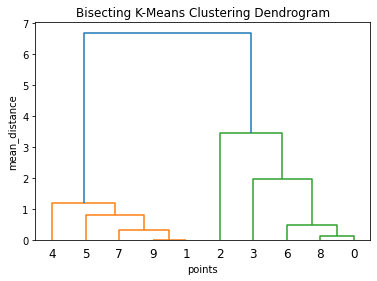
\includegraphics[width=0.33\textwidth,height=\textheight]{img/dengrogram-example.png}
\caption{Bsp. eines Dendrogramms}
\end{figure}

Der größte Nachteil dieser Verfahren ist die Laufzeit. Meistens liegt
diese bei mindestens \(\mathcal{O}(n^2)\) bis teilweise
\(\mathcal{O}(n^3)\). \autocite{dogan2022}

Deshalb entwickelten Steinbach et al. \autocite{steinbach2000} den
\emph{Bisecting K-Means-Algorithmus}. Dabei handelt sich um ein
Top-down-Clustering-Verfahren, welches für den Split eines größeren
Clusters in zwei kleinere den K-Means mit \(k=2\) benutzt. Da nur das
initiale Cluster alle Datenpunkte enthält und mit den folgenden Splits
die Cluster immer kleiner werden, ist die Laufzeit linear
(\(\mathcal{O}(n)\))

\hypertarget{bisecting-k-prototypes}{%
\section{Bisecting K-Prototypes}\label{bisecting-k-prototypes}}

\hypertarget{herleitung}{%
\subsection{Herleitung}\label{herleitung}}

Für die beschriebenen möglichen Anwendungen der Clusteranalyse in
PIM-Systemen sind hierarchische Verfahren zu bevorzugen, da die
ineinander verschachtelte Cluster-Hierarchie eine umfassendere Analyse
ermöglicht \autocite{dogan2022}. Außerdem entfällt eine vorherige
Bestimmung der erwarteten Anzahl an Clustern, wie sie partitionierende
Verfahren benötigen.

Gleichzeitig ist die quadratische oder noch schlechtere Laufzeit vieler
hierarchischer Verfahren problematisch. Produktkataloge umfassen gerne
mehrere tausend oder sogar einige Millionen Produkte, sodass eine
möglichst geringe Laufzeit zu bevorzugen ist.

Der naheliegendste Ansatz besteht nun darin, den Bisecting
K-Means-Algorithmus zu verwenden. Allerdings kann dieser nur numerische
Vektoren verarbeiten. Grundsätzlich können kategoriale Werte in
numerische umgewandelt werden (z.B. durch Nummerierung also Rot = 1,
Grün = 2, Blau = 3). Solche Umwandlungen verzerren aber das Datenset
(rote und blaue Produkte unterscheiden sich nun stärker voneinander als
rote und grüne). \autocite[Kap. 1.2.6 Mixed Variables]{kaufman2009}

Schließlich wurde zur Lösung die Grundidee des Bisecting K-Means mit dem
K-Prototypes-Algorithmus kombiniert. Das Clustering erfolgt also nach
dem Ablauf des Bisecting K-Means, allerdings wird für den Zweier-Split
eines großen Clusters in zwei kleineren stattdessen der
K-Prototypes-Algorithmus verwendet. Das daraus resultierende Verfahren
\emph{Bisecting K-Prototypes} ist ein hierarchisches
Top-down-Clustering-Verfahren für gemischte Datensets mit linearer
Laufzeit.

\hypertarget{erweiterungen}{%
\subsection{Erweiterungen}\label{erweiterungen}}

\hypertarget{fehlende-werte}{%
\subsubsection{fehlende Werte}\label{fehlende-werte}}

Mit dem Bisecting K-Prototypes lassen sich bereits viele Attribute der
Produkte in PIM-Systemen für das Clustering verwenden. Klassische
Implementierungen von Clustering-Verfahren können allerdings nicht mit
fehlenden Werten umgehen \autocite[siehe z.B.][]{sklearn2022}. Füllt man
diese mit einem Pseudowert (z.B. dem Mittelwert), so werden die
Datensets wieder verzerrt. In PIM-Systemen kommen häufig Produkte aus
verschieden Kategorien mit dadurch sehr unterschiedlichen Attributen
vor. Dadurch weisen die meisten Produkte in den meisten Attributen
keinen Wert auf. Eine gesonderte Betrachtung fehlender Werten ist also
vonnöten.

Die folgende Formel zeigt die Distanzfunktion, welche für das Clustering
verwendet wurde:

\begin{align}
    d(x_1, x_2) &= \frac{\sum d'(x_1^i, x_2^i)}{|x_1^{\text{non }null} \cup x_2^{\text{non }null}|} \\
    d'(x_1^i, x_2^i) &= \begin{cases}
        0 &, x_1^i \text{ is } null \wedge x_2^i \text{ is } null \\
        1 &, x_1^i \text{ is } null \vee x_2^i \text{ is } null \\
        |x_1^i - x_2^i| &, i \text{ is } numerical \\
        0 &, i \text{ is } categorical \wedge x_1^i = x_2^i \\
        1 &, i \text{ is } categorical \wedge x_1^i \neq x_2^i
    \end{cases}
\end{align}

Zwei Produkte werden Attribut für Attribut miteinander verglichen. Dabei
liegt der Abstand für jedes Paar von Attributwerten im Interval
\([0,1]\). Die Abstände auf Basis der einzelnen Attribute werden
anschließend summiert und durch die Menge an Attributen geteilt. Dadurch
liegt der Abstand zweier Produkte insgesamt ebenfalls im Interval
\([0,1]\).

Weisen beide Produkte in einem Attribut keinen Wert auf, so wird dieses
sowohl über als auch unter dem Bruchstrich ignoriert. Fehlt der Wert nur
bei einem der beiden Produkte, so wird der maximale Abstand von \(1\)
addiert. Dieses Vorgehen ist durch den Jaccard-Koeffizienten inspiriert,
welcher für asymmetrische binäre Attribute verwendet wird. Er ignoriert
ebenfalls alle Attribute, bei denen beide Werte \(false\) sind.
\autocite[siehe][Kap. 1.2.4 Binary Variables]{kaufman2009}

Die numerischen Attribute werden mittels Manhattan-Abstand verrechnet.
Damit auch hier die Abstände auf Attributebasis im Interval \([0,1]\)
liegen, müssen die Werte vorher auf ebendieses Interval skaliert werden.
Eine solche Normalisierung sorgt außerdem dafür, dass alle Attribute in
etwa das gleiche Gewicht zueinander haben. \autocite[Kap. 1.2.1
Interval-Scaled Variables]{kaufman2009}

Die kategorialen Attribute werden nach dem Prinzip des Simple Matchings
verarbeitet. Weisen beide Produkte den gleichen Wert auf, so wird \(0\)
und im Falle von Ungleichheit \(1\) addiert.

\hypertarget{multi-kategoriale-attribute}{%
\subsubsection{Multi-kategoriale
Attribute}\label{multi-kategoriale-attribute}}

Eine weitere Form von Attributen in PIM-Systemen sind sog.
Multi-Select-Felder. Das sind Attribute, wo eine Liste an
Auswahlmöglichkeiten definiert wird. Anschließend kann für ein Produkt
ein oder mehrere dieser Optionen ausgewählt werden. Dies könnte z.B. die
Farbe sein, da Produkte auch mehrfarbig sein können.

Diese Attribute könnten zum einen in einfache kategoriale Attribute
umgewandelt werden, indem die gewählten Optionen sortiert und mittels
Kon­ka­te­na­ti­on verbunden werden. Dadurch würden sich aber zwei Produkte,
die z.B. \(\{\text{Rot}\}\) und \(\{\text{Rot},\text{Grün}\}\) sind,
maximal voneinander unterscheiden.

Daher wurde ein alternativer Ansatz erdacht und die Distanzfunktion wie
folgt erweitert:

\begin{equation}
d'(x_1^i, x_2^i) = \begin{cases}
    ... \\
    1 - \frac{|x_1^i \cap x_2^i|}{|x_1^i \cup x_2^i|} &, i \text{ is } multi-categorical
\end{cases}
\end{equation}

Diese multi-kategorialen Attribute werden mit einem ``inversen
Jaccard-Koeffizient'' verrechnet. Normalerweise wird der
Jaccard-Koeffizient zur Bewertung der Ähnlichkeit zweier Produkte als
ganzes verwendet. Hier wird für jedes multi-kategoriale Attribut der
Jaccard-Koeffizient für die Werte des jeweiligen Attributes einzeln
berechnet und aufaddiert.

\hypertarget{string-attribute}{%
\subsubsection{String-Attribute}\label{string-attribute}}

Schließlich gibt es noch Freitext-Felder in den Produktdaten wie z.B.
den Produkttitel. Dies sind keine klassischen kategoriale Werte, da kaum
ein Wert dem anderen gleicht. \autocite{rajalingam2011}

Zur Verarbeitung werden die Strings zunächst in Tokens zerlegt
(Tokenization), ihre Endungen entfernt (Stemming) und schließlich
Stop-Words entfernt (Stop-Word-Removal) -- alles typische
Verarbeitungsschritte aus dem Document Retrieval \autocite{cohen2003}.
Aus einem Titel wie ``Samsung Galaxy S20 128GB'' wird nun
\(\{\text{samsung}, \text{galaxi}, \text{s20}, \text{128gb}\}\).

Durch die Umwandlung in Tokens, sind die String-Attribute equivalent zu
den multi-kategorialen Attributen und können mit dem gleichen Verfahren
verarbeitet werden.

\hypertarget{experimentelle-uxfcberpruxfcfung}{%
\section{Experimentelle
Überprüfung}\label{experimentelle-uxfcberpruxfcfung}}

\hypertarget{uxfcberblick}{%
\subsection{Überblick}\label{uxfcberblick}}

Für die praktische Evaluation ist Akeneo-PIM \autocite{akeneo2022about}
(ein Open-Source PIM-System mit weiter Verbreitung) verwendet worden.
Dieses System wurde mit Produkten aus dem sehr umfangreichen
Online-Katalog Icecat \autocite{icecat2021} gefüllt, wo Hersteller aus
der ganzen Welt ihre Produktdatenblätter für die Verteilung an Händler
hochladen.

Anschließend wurde das hergeleitete Clustering-Verfahren implementiert.
Nun wurde das Datenset geclustert, wobei verschiedene Kombinationen an
Attributen für das Clustering verwendet worden sind. Diese
Clustering-Ergebnisse wurde schließlich mittels einiger Metriken
evaluiert.

\hypertarget{datenset}{%
\subsection{Datenset}\label{datenset}}

Es wurden 42 Smartphones der Samsung Galaxy S-Reihe importiert. Dabei
waren 17 Smartphones der Generation S20, 21 der Generation S21 und 4 der
Generation S22 vertreten. Es wurden sowohl Modelle der
Produktausführungen Standard, Plus und Ultra sowie der sog. Fan Edition
(FE) importiert. Die Smartphones zeichnen sich durch ein große Menge an
verschiedenen Attributen der unterschiedlichsten Typen aus. Die folgende
Tabelle gibt eine Übersicht dazu:

\begin{longtable}[]{@{}lrrrl@{}}
\caption{Übersicht zu den Attributen der 42 Smartphones}\tabularnewline
\toprule()
Typ & Anzahl & Ø non-\texttt{null} & Ø unique & Beispiele \\
\midrule()
\endfirsthead
\toprule()
Typ & Anzahl & Ø non-\texttt{null} & Ø unique & Beispiele \\
\midrule()
\endhead
numerisch & \(56\) & \(21.8\) & \(3.7\) & Weight, Width, Depth,
Height \\
kategorial & \(106\) & \(28.2\) & \(1.3\) & OS installed, SIM Card
Type \\
multi-kat. & \(22\) & \(25.2\) & \(3.5\) & Product Color, 3G
standards \\
String & \(11\) & \(28.4\) & \(13.5\) & Title, Description \\
\emph{alle:} & \emph{195} & \emph{25.9} & \emph{2.9} & \\
\bottomrule()
\end{longtable}

Die Spalte ``Anzahl'' zeigt, wie viele Attribute je Typ vorkommen. Die
numerischen und kategorialen Attribute dominieren hierbei das Datenset.
Die Spalte ``Ø non-\texttt{null}'' zeigt, wie viele der 42 Produkte im
Schnitt in diesem Typ einen Wert aufweisen. Es kommen also fast so viele
fehlende wie gefüllte Werte vor. Die Spalte ``Ø unique'' gibt an, wie
viele verschiedene Wertausprägungen im Schnitt in der jeweiligen
Attributart vorkommen. Die Strings weisen hierbei die höchste Menge an
unterschiedlichen Werten auf, was in der Natur dieses Types liegt.
Aufgrund des recht kleinen Datensets mit vielen ähnlichen Produkten, ist
die Variation an Werten gering.

\hypertarget{evaluation-metriken}{%
\subsection{Evaluation \& Metriken}\label{evaluation-metriken}}

Für die Bewertung des Clustering-Verfahrens sind verschiedene Metriken
verwendet worden:

Die \textbf{Stabilität} zeigt die Übereinstimmung der
Clustering-Ergebnisse von zehn verschiedenen Durchläufen des Bisecting
K-Prototypes. Da das Verfahren mit zufälligen Startpunkten arbeitet,
sind die Ergebnisse von zwei Durchläufe nicht immer deckungsgleich. Ein
sinnvolles Clustering-Verfahren sollte aber dennoch einen gewissen
Determinismus aufweisen. Die Übereinstimmung der Clusterings wurde
mittel Adjusted-Rand-Index \autocite{hubert1985} berechnet. Er liefert
Werte zwischen \(-1\) und \(1\) und je höher er liegt, desto höher ist
die Übereinstimmung zweier Cluster-Zuteilungen.

Die \textbf{Qualität} wird mittels des Silhouetten-Koeffizienten
\autocite{rousseeuw1987} gemessen. Er berechnet den durchschnittlichen
Abstand der Datenpunkte zu den Punkten im selben Cluster im Verhältnis
zu den Punkten des unmittelbar benachbarten Clusters. Auch hier können
Werte zwischen \(-1\) und \(1\) entstehen. Je näher an \(1\), desto
besser sind die Cluster voneinander getrennt.

Mit der \textbf{Erkennung} wird geprüft, ob das Clustering-Verfahren die
inhärenten Strukturen des Datensets erkennen kann. Die Smartphones
stammen aus drei verschiedenen Generationen und es gibt elf verschiedene
Modelle (unter Berücksichtigung der Generationen). Auf der
Hierarchiestufe \(k=3\) sollten also die Smartphones der gleichen
Generationen dem gleichen Cluster zugeordnet werden. Ebenso bei \(k=11\)
für die Smartphone-Modelle. Die Übereinstimmung der berechneten
Cluster-Zuteilung mit der erwarteten wurde mittels Adjusted-Rand-Index
berechnet.

Schließlich befinden sich im Datenset sechs Paare an \textbf{Duplikaten}
-- also das gleiche Produkt unter verschiedenen Ids. Ein hierarchisches
Clustering-Verfahren sollte die Duplikate stets in die gleichen Cluster
sortieren und erst beim letzten Split die Duplikate schließlich
voneinander trennen. Ist dies der Fall, so wird ein Duplikate als
erfolgreich erkannt gezählt.

\hypertarget{auswertung}{%
\section{Auswertung}\label{auswertung}}

Die folgende Tabelle zeigt die Ergebnisse des Clustering für
verschiedene (ausgewählte) Kombinationen an Attributen. Im Versuch
``Strings'' sind nur die String-Attribute für das Clustering benutzt
worden -- bei ``num+kat'' die numerischen und kategorialen Attribute.
Alle weiteren Versuche (mit ``+'' beginnend) haben die numerischen und
kategorialen um multi-kategoriale (mul) oder die String-Attribute (str)
erweitert. Im Versuch ``mul\_k'' sind die multi-kategorialen Attribute
nicht nach dem hergeleiteten Verfahren verarbeitet, sondern in einfache
kategoriale Attribute umgewandelt worden.

\begin{longtable}[]{@{}
  >{\raggedright\arraybackslash}p{(\columnwidth - 14\tabcolsep) * \real{0.1176}}
  >{\raggedleft\arraybackslash}p{(\columnwidth - 14\tabcolsep) * \real{0.1176}}
  >{\raggedleft\arraybackslash}p{(\columnwidth - 14\tabcolsep) * \real{0.1176}}
  >{\raggedleft\arraybackslash}p{(\columnwidth - 14\tabcolsep) * \real{0.1176}}
  >{\raggedleft\arraybackslash}p{(\columnwidth - 14\tabcolsep) * \real{0.1176}}
  >{\raggedleft\arraybackslash}p{(\columnwidth - 14\tabcolsep) * \real{0.1176}}
  >{\raggedleft\arraybackslash}p{(\columnwidth - 14\tabcolsep) * \real{0.1176}}
  >{\raggedleft\arraybackslash}p{(\columnwidth - 14\tabcolsep) * \real{0.1765}}@{}}
\caption{Ergebnisse des Clustering}\tabularnewline
\toprule()
\begin{minipage}[b]{\linewidth}\raggedright
Versuch
\end{minipage} & \begin{minipage}[b]{\linewidth}\raggedleft
Stabilität
\end{minipage} & \begin{minipage}[b]{\linewidth}\raggedleft
Qualität
\end{minipage} & \begin{minipage}[b]{\linewidth}\raggedleft
\end{minipage} & \begin{minipage}[b]{\linewidth}\raggedleft
\end{minipage} & \begin{minipage}[b]{\linewidth}\raggedleft
Erkennung
\end{minipage} & \begin{minipage}[b]{\linewidth}\raggedleft
\end{minipage} & \begin{minipage}[b]{\linewidth}\raggedleft
Duplikate
\end{minipage} \\
\midrule()
\endfirsthead
\toprule()
\begin{minipage}[b]{\linewidth}\raggedright
Versuch
\end{minipage} & \begin{minipage}[b]{\linewidth}\raggedleft
Stabilität
\end{minipage} & \begin{minipage}[b]{\linewidth}\raggedleft
Qualität
\end{minipage} & \begin{minipage}[b]{\linewidth}\raggedleft
\end{minipage} & \begin{minipage}[b]{\linewidth}\raggedleft
\end{minipage} & \begin{minipage}[b]{\linewidth}\raggedleft
Erkennung
\end{minipage} & \begin{minipage}[b]{\linewidth}\raggedleft
\end{minipage} & \begin{minipage}[b]{\linewidth}\raggedleft
Duplikate
\end{minipage} \\
\midrule()
\endhead
& & \emph{Ø} & \(k=3\) & \(k=11\) & \(k=3\) & \(k=11\) & \\
Strings & 0.91 & 0.34 & 0.26 & 0.40 & 0.64 & \textbf{0.87} & \textbf{6 /
6} \\
num+kat & \textbf{0.98} & \textbf{0.43} & 0.31 & \textbf{0.60} &
\textbf{0.65} & 0.71 & 5 / 6 \\
+mul & \textbf{0.98} & 0.41 & \textbf{0.37} & 0.57 & 0.16 & 0.70 & 5 /
6 \\
+mul\_k & 0.97 & 0.40 & 0.30 & 0.53 & 0.52 & 0.68 & 5 / 6 \\
+str & \textbf{0.98} & 0.41 & 0.30 & 0.58 & \textbf{0.65} & 0.66 & 5 /
6 \\
+mul+str & 0.92 & 0.39 & 0.35 & 0.56 & 0.16 & 0.70 & \textbf{6 / 6} \\
\bottomrule()
\end{longtable}

Die Stabilität und die Erkennung von Duplikaten erreicht für alle
Versuche sehr hohe Werte.

Die Erkennung von Smartphone-Generationen (\(k=3\)) ist mit Werten
zwischen \(0.16\) und \(0.65\) eher mittelmäßig. Die Smartphone-Modelle
(\(k=11\)) erreichen höhere Werte zwischen \(0.66\) und \(0.87\).
Abbildung \ref{fig:result} zeigt das Dendrogramm zum Clustering mit
numerischen und kategorialen Attributen. Hier wird deutlich, dass die
Trennung in die Generationen S20 und S21 sehr gut funktioniert. In der
Gruppe mit den S22-ern (orange) finden sich hingegen auch Smartphones,
die nicht in diese Generation gehören.

\begin{figure}
\centering
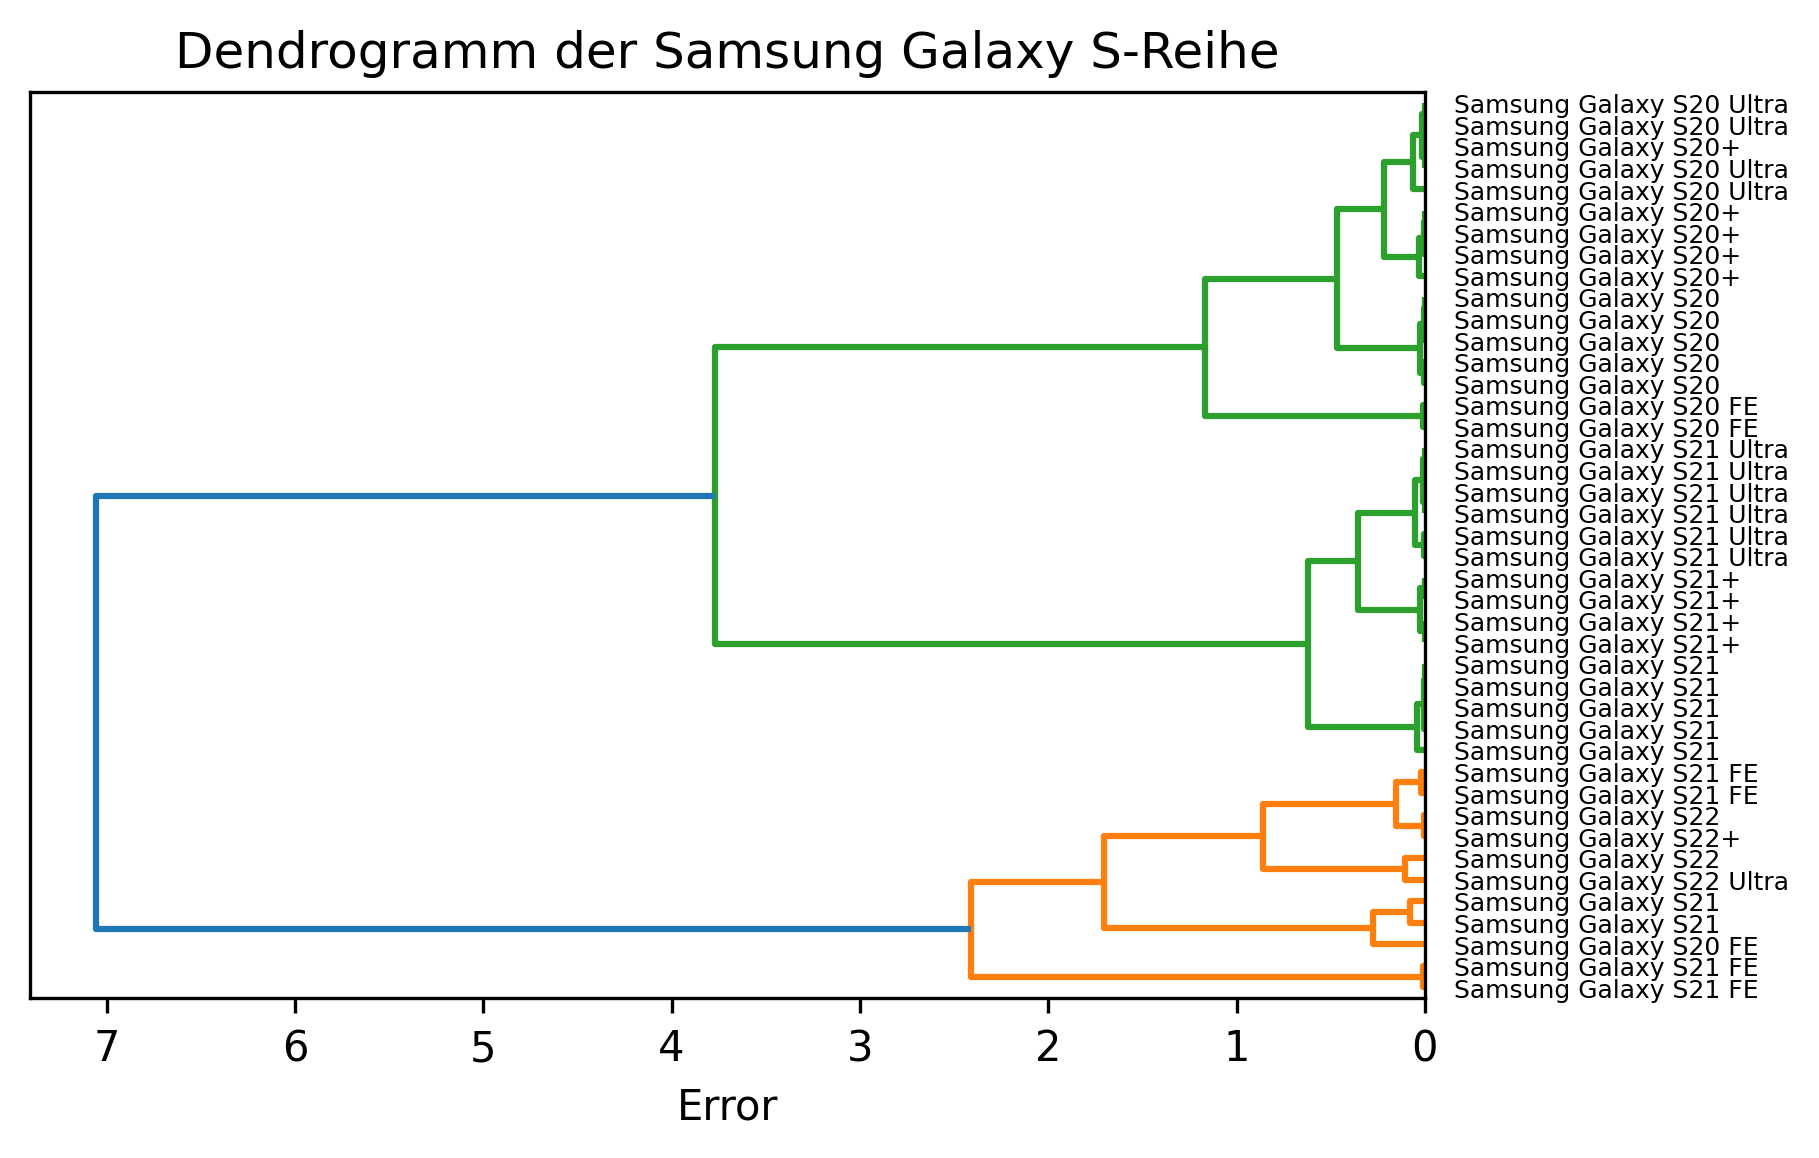
\includegraphics[width=0.8\textwidth,height=\textheight]{img/dendrogram-phones.png}
\caption{Ergebnis des Clustering mit nur numerischen und kategorialen
Attributen \label{fig:result}}
\end{figure}

Die Qualität ist einmal als Durchschnitt für alle möglichen Werte von
\(k\) gegeben sowie für die beiden relevanten Hierarchiestufen. Sie
liegt in allen Versuchen eher in mittelmäßigen Bereichen zwischen
\(0.26\) und \(0.60\). Dies könnte daran liegen, dass sich die Produkte
des Datensets insgesamt ziemlich ähnlich sind (alle vom gleichen
Hersteller, recht geringe Anzahl an verschiedenen Wertausprägungen).

Auffällig bei den Versuchen ist, dass die ausschließliche Verwendung von
numerischen und kategorialen Attributen auf fast allen Metriken die
besten Werte liefert. Die Hinzunahme von multi-kategorialen und
String-Attributen hingegen verschlechtert diese Ergebnisse wieder.

Die Verarbeitung der multi-kategorialen Attribute nach dem hergeleiteten
Verfahren (+mul) bringt etwas bessere Stabilität und Qualität als die
Umwandlung in einfache kategoriale Attribute (+mul\_k). Die Erkennung
der Generationen ist mit dem hergeleiteten Verfahren drastisch
schlechter. Die Modelle werden dann wiederum etwa gleich gut erkannt.
Insgesamt haben die multi-kategorialen Attribute keinen positiven
Einfluss auf das Clustering. Eine klare Überlegenheit des hergeleiteten
Verfahrens zur Umwandlung in einfache kategoriale Attribute ist
ebenfalls nicht erkennbar.

Die String-Attribute mit den numerischen und kategorialen Attributen zu
kombinieren verschlechtert die Clustering-Ergebnisse. Werden allerdings
nur die String-Attribute verwendet, so liefern sie adäquate Cluster.
Zwar ist die Qualität dieser Cluster im Vergleich sehr schlecht, aber
vor allem die Erkennung und die Duplikate erreichen etwas bessere Werte
als die Kombination aus numerischen und kategorialen Attributen. Dies
lässt sich dadurch erklären, dass z.B. im Produkttitel die wesentlichen
Informationen des Produktes komprimiert -- wenn auch unstrukturiert --
hinterlegt sind.

\hypertarget{fazit-und-ausblick}{%
\section{Fazit und Ausblick}\label{fazit-und-ausblick}}

In diesem Paper wurde ein hierarchisches Clustering-Verfahren für
gemischte Datensets mit linearer Laufzeit hergeleitet: \emph{Bisecting
K-Prototypes}. Das Verfahren wurde erweitert, um ohne Verzerrung der
Daten mit fehlenden Werten (\texttt{null}-Values) umgehen zu können. In
der anschließenden praktischen Evaluation zeigte sich, dass das
Verfahren funktioniert und sinnvolle Cluster für ein Datenset mit recht
komplexen Datenpunkten (Smartphones mit über 100 verschiedenen
Attributen) finden kann.

Es ist außerdem eine Erweiterung des Verfahrens für sog.
multi-kategoriale Attribute vorgestellt worden, welche sich ebenfalls
für String-Attribute verwenden lässt. In der praktischen Evaluation hat
die Hinzunahme dieser Attributtypen die Cluster allerdings nicht
verbessert. Werden ausschließlich String-Attribute für das Clustering
verwendet, so entstehen ähnlich gute Cluster wie mit ausschließlich
numerischen und kategorialen Attributen. U.U. ist das hergeleitete
Verfahren besonders für die Verarbeitung von Datensets geeignet, welche
aus Freitext-Feldern bestehen. Hier könnte zukünftige Forschung
anknüpfen.

Es ist wichtig zu beachten, dass das verwendete Datenset für die
Evaluation sehr klein gewesen ist und eine sehr beschränkte Auswahl an
Produkten enthalten hat. Alle Ergebnisse dieser Arbeit sind also
bestenfalls als vorläufig anzusehen und sollten in Zukunft mit weiteren
Datensets überprüft werden. Speziell sollte dabei geprüft werden, ob die
multi-kategorialen Attribute in anderen Datensets einen positiven
Einfluss auf das Clustering haben.

Weitere Versuche in der Zukunft könnten den Bisecting K-Prototypes mit
alternativen Verfahren vergleichen. Im Speziellen wäre hier ein
Vergleich der nötigen Vorverarbeitungen der Datensets für die
verschiedenen Verfahren und deren Einfluss auf die Cluster-Ergebnisse
interessant.

Erweisen sich diese Versuche als erfolgreich, so könnte mit dem
Bisecting K-Prototypes ein solides, effizientes und flexibles Verfahren
für das hierarchische Clustern einer Vielzahl von Datensets gefunden
worden sein.
